\section{Implementacja}
Implementacja projektu, ze względu na rodzaj przedsięwzięcia został podzielona na dwie niezależne części.

Część kliencka, wysyłająca zapytania, odbierająca odpowiedzi na zapytania oraz odbierająca stan gry. Część kliencka odpowiedzialna jest również za rysowanie aktualnego stanu gry oraz interfejsu użytkownika.

Część serwerowa wykonująca wszystkie obliczenia, odbierająca zapytania, przetwarzająca je i rozsyłając je do użytkowników.

W rozdziale tym przedstawiono również specyfikację protokołu wykorzystywanego do komunikacji między stacją klienta a serwerem.

\subsection{Model obiektowy}
W niniejszym podrozdziale przedstawiono schemat obiektów zaimplementowany w aplikacji. Rysunek \ref{fig:main-obj} przedstawia diagram głównej część obiektów modelujących system, na rysunku \ref{fig:misc-obj} natomiast, pokazano obiekty, nie mające bezpośredniej relacji z główną częścią części serwerowej.
\begin{figure}[ht]
    \centering
    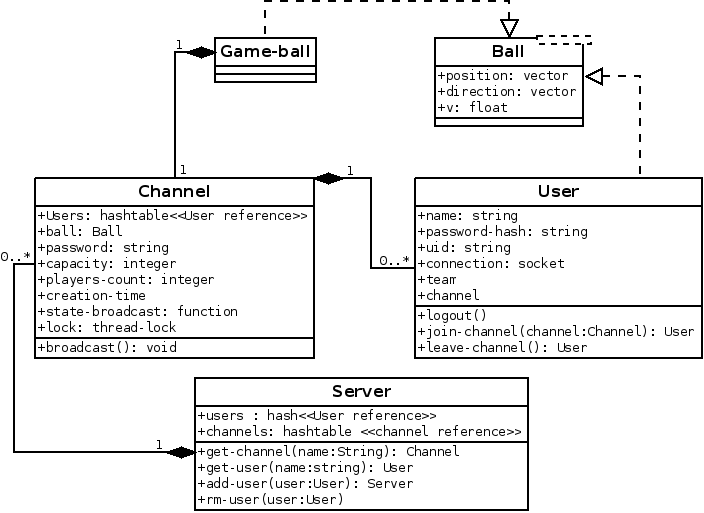
\includegraphics[width=0.8\textwidth]{imgs/main-obj.png}
    \caption{Diagram obiektów głównej części systemu.}
    \label{fig:main-obj}
\end{figure}

\begin{figure}[ht]
    \centering
    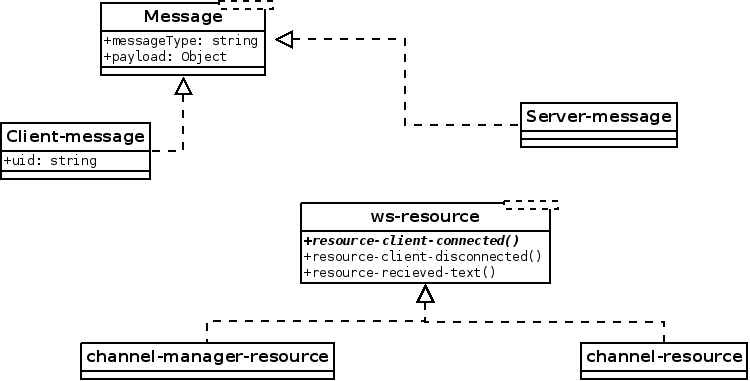
\includegraphics[width=0.8\textwidth]{imgs/misc-obj.png}
    \caption{Diagram pozostałych obiektów.}
    \label{fig:misc-obj}
\end{figure}

Ze względu na charakter działania części klienckiej, która nie przechowuje żadnego stanu, nie został zaimplementowany żaden konkretny model obiektowy.

\subsection{Protokół komunikacyjny}

Korzystając z aplikacji tworzonych z wykorzystaniem języka JavaScript, nie sposób wykorzystać pełnie jego możliwości bez znajomości JSON. JSON jest notacją reprezentacji obiektów w języku, nie tylko JavaScript, ale wszystkie tych, które dostarczają możliwość obsługi tego standardu, który opiera się na prostym, hierarchicznym formacie tekstowym.

Wsparcie dla JSON w języku JavaScript jest zapewnione dzięki bibliotece standardowej, w języku Common Lisp należy wykorzystać pakiet \emph{CL-JSON}. Rysunek \ref{fig:jsonexample} przedstawia przykładowy obiekt w notacji JSON.
\begin{figure}[ht]
    \centering
    \begin{verbatim}
      {
        name : "Jan",
        lastName : "Kowalski",
        emails : [jan@kowalski.pl, janek@games.com],
        pet :
        {
          name : "reksio",
          species "C. Lupus",
          age: 4
        }
     }
      \end{verbatim}
    \caption{Przykładowa reprezentacja obiektu w formacie JSON}
    \label{fig:jsonexample}
\end{figure}
W przypadku prostych protokołów, z łatwością można wykorzystać JSON w zastępstwie za XML.

W przypadku zaimplementowanego projektu, komunikaty dzielą się na dwa typy:
\begin{itemize}
  \item Wiadomości klienta (\emph{client message}).
  \item Wiadomości serwera (\emph{server message}).
\end{itemize}

\subsubsection{Wiadomość klienta}
Ogólna budowa żądań klienta została przedstawiona na rysunku \ref{fig:jsonclient}.
\begin{figure}[ht]
    \centering
    \begin{verbatim}
      {
        userId: <<ID klienta lub NULL>>,
        messageType: <<Rodzaj rządania>>,
        payload: <<obiekt wymagany przez typ wiadomości>
      }
      \end{verbatim}
    \caption{Reprezentacja obiektu zapytania klienta w notacji JSON.}
    \label{fig:jsonclient}
\end{figure}
Dozwolone żądań, wraz z opisem i wymaganym obiektem zostały przedstawione w tabeli \ref{tab:clientmessagestypes}

\begin{table}[h]
  \centering
  \begin{tabular}{ |p{1.5cm}|p{6cm}|p{6cm}| }
    \hline
    \textbf{Typ wiadomości} & \textbf{Opis} & \textbf{Rodzaj obiektu} \\ \hline
    login & Próba zalogowania użytkownika & Obiekt przesyłający nazwę użytkownika oraz skrót SHA1 jego hasła. \\
    create & Utwórz kanał gry & Obiekt podobny do obiektu \emph{channel}. Z wymaganymi polami \emph{name} i {capacity} oraz opcjonalnym polem \emph{password}. \\
    register & Zarejestrowanie użytkownika & Tożsame z wiadomością typu login \\
    join & Dołącz do rozgrywki & Obiekt zawierający nazwę porządnego kanału \\
    event & Wydarzenie jakie zostało wygenerowane przez użytkownika & Typ wydarzenia, np. naciśnięcie lewej strzałki, spacji itp. \\
    list & Pobierz listę wszystkich dostępnych kanałów na serwerze & ignorowane \\
    logout & Wylogowanie użytkownika & ignorowane \\
    \hline
  \end{tabular}
  \caption{Przydział prac poszczególnym członkom zespołu}
  \label{tab:clientmessagestypes}
\end{table}
\subsubsection{Wiadomość serwera}
Wiadomości serwera można podzielić na dwie grupy:
\begin{itemize}
  \item Odpowiedzi na zadania.
  \item Cyklicznie rozsyłany stan rozgrywki (do wszystkich użytkowników na danym kanale).
\end{itemize}

Odpowiedź na żądanie ma format tożsamy z formatem wiadomości klienta z tym, że pole \emph{messageType} może przyjąć jedną z dwóch wartości \emph{ok} lub \emph{error} a pole \emph{uid} jest nieobecne. W przypadku \emph{ok}, pole \emph{payload} niesie wartość wyniku żądania klienta. Jeżeli pole \emph{messageType} ma wartość \emph{error} serwer, pole \emph{payload} zawiera obiekt przedstawiony na rysunku \ref{fig:errors}
\begin{figure}[ht]
    \centering
    \begin{verbatim}
      {
        errorCode : <<Numer>>,
        errorDescription : <<Opis błędu>>
      }
      \end{verbatim}
    \caption{Reprezentacja obiektu zapytania klienta w notacji JSON.}
    \label{fig:errors}
\end{figure}

Stan rozsyłany do użytkowników zawiera następujące pola, opisane w tabeli \ref{tab:state-fields}.

\begin{table}[ht]
  \centering
  \begin{tabular}{ |p{3cm}|p{8cm}| }
    \hline
    \textbf{Nazwa pola} & \textbf{Opis} \\ \hline
    \emph{players} & Lista użytkowników na kanale, łącznie z ich pozycją, rotacją i przynależnością do drużyny \\
    \emph{scoreYellow} & Punkty drużyny żółtej \\
    \emph{scoreBlue} & Punkty drużyny niebieskiej \\
    \emph{ballInstance} & Pozycja piłki \\
    \hline
  \end{tabular}
  \caption{Przydział prac poszczególnym członkom zespołu}
  \label{tab:state-fields}
\end{table}

\subsection{Cześć serwerowa}
Implementacja serwera, za sprawą wykorzystania języka Common Lisp została zaprogramowana korzystając z dwóch paradygmatów programowania. Funkcyjnym, za sprawą natury języka Lisp i obiektowym, za sprawą CLOS\footnote{\url{https://en.wikipedia.org/wiki/Common_Lisp_Object_System}}.

Przepływ danych w funkcjach jest następujący:
\begin{enumerate}
\item Dane od klienta docierają do funkcji obsługującej dane przychodzące od klientów. Funkcja jest implementacją funkcji \emph{resource-received-text} interfejsu \emph{ws-resource}.
\item Ponieważ wiadomość jest zserializowana do postaci tekstowej, sformatowanej do notacji JSON\footnote{\url{http://www.json.org/}}, należy ją zdeserializować korzystając z funkcji \emph{json-to-client-message}. W zależności od wartości pola \emph{messageType} wiadomość zostanie zserializowana do dane obiektu CLOS. Informacje o tym, jaki typ obiektu wybrać znajdują się w liście asocjacyjnej \emph{*message-payload-alist*}.
\item Obiekt zwrócony przez poprzednią funkcję trafia do funkcji \emph{dispatch-message}, która również w zależności od \emph{messageType} wywołuje odpowiednią funkcję obsługującą zapytanie.
\item Funkcja obsługująca zapytanie zwraca tzn. listę własności (\emph{property list}) definiującą wynik obsługi zdarzenia. Lista następnie trafia do funkcji \emph{response-with} która serializuje listę do obiektu \emph{server-message} definiującą rodzaj odpowiedzi, wynik lub ewentualny kod błędu w przypadku niepowodzenia.
\item Obiekt jest następnie serializowana do JSON i wysyłana do klienta korzystając z funkcji \emph{write-to-client-text}.
\end{enumerate}
Rysunek \ref{fig:serverflow} wizualizuje proces przetwarzania zapytań przez serwer.

Ponieważ serwer obsługuje szereg kanałów, jak i wielu użytkowników oraz oba te obiekty są zmienne w ilości, należy przechowywać je w kontenerach. Podstawowym kontenerem jest lista, jednak oczywiście złożoność dodawania, wyszukiwania oraz innych operacji jest zbyt wysoko. Aby rozwiązać ten problem wykorzystano strukturę tablicy haszującej dostępnej w bibliotece standardowej języka Common Lisp.
\begin{figure}[ht]
    \centering
    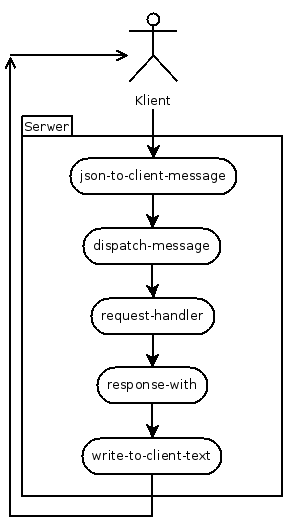
\includegraphics[width=0.5\textwidth]{imgs/serverflow.png}
    \caption{Przepływ danych po stronie serwerowej aplikacji.}
    \label{fig:serverflow}
\end{figure}

\subsection{Cześć kliencka}
Struktura interfejsu użytkownika, zdefiniowana przy użyciu języka HTML, reaguje na akcje użytkownika korzystając z języka JavaScript. Funkcje obsługujące zdarzenia połączone są z przyciskami korzystając z biblioteki jQuery\footnote{\url{http://jquery.com/}}. Na uwagę zasługuje funkcja \emph{dispatch}, która jest wysyłana za każdym razem gdy dane są zwracane od serwera. Funkcja, w zależności od tego jaka funkcja została wywołana przez interfejs użytkownika, wywoła funkcję która obsługuje odpowiedź na zapytanie. Jeżeli serwer odpowie wiadomością sugerującą niepowodzenie w realizacji żądania wysłanego przez klienta, funkcja obsługująca odpowiedź nie zostanie wywołana, a jedynie zostanie przedstawiona wiadomość z opisem błędu na interfejsie użytkownika.

Rysunek \ref{fig:clientflow} prezentuje, jak wygląda proces przetwarzania akcji klienta.

\begin{figure}[ht]
    \centering
    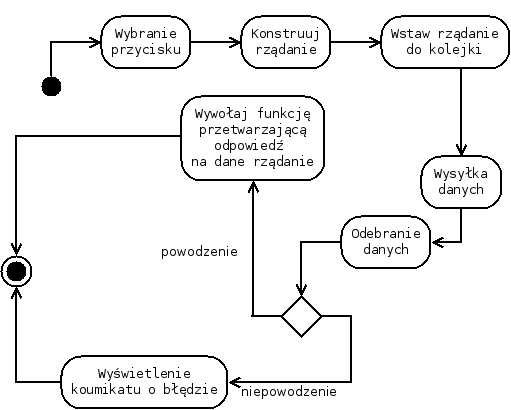
\includegraphics[width=0.6\textwidth]{imgs/clientflow.png}
    \caption{Poszczególne aktywności generowane podczas przetwarzania danych klienta.}
    \label{fig:clientflow}
\end{figure}
